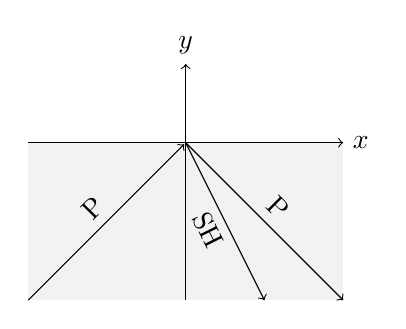
\begin{tikzpicture}
 \fill[black!5!white] (-2,0) rectangle (2,-2);
 \draw[->] (-2,0 ) -- (2,0) node[right] {$x$};
 \draw[->] ( 0,-2 ) -- (0,1) node[above] {$y$};
 \draw[->] (-2,-2) -- node[above, sloped] {P} (-0.02,-0.02);
 \draw[->] (0,0) -- node[below, sloped] {SH} (1, -2);
 \draw[->] (0,0) -- node[above, sloped] {P} (2, -2);
\end{tikzpicture}


In einem linear elastischen, isotropen Kontinuum (Elastizitätsmodul $E$ und Querkontraktionszahl $\nu$ trifft eine P-Welle
\begin{equation*}
\mathbf{u}_1(\mathbf{r},t)=\mathbf{n}_1 A_1 \cos\bigl(\kappa_1 (\mathbf{n}_1\cdot \mathbf{r}-c_\mathrm{P}t)\bigr) 
\quad \text{mit} \quad
\mathbf{u}=[u_1,v_1,w_1]^\mathrm{T}
\quad \text{und} \quad
\mathbf{r}=[x,y,z]^\mathrm{T}
\end{equation*}
auf einen festen Rand. Die entsprechende Randbedingung lautet
\begin{equation*}
\sigma_{xy}(\mathbf{r}_\mathrm{R},t) = \sigma_{yy}(\mathbf{r}_\mathrm{R},t) = 0
\quad \text{mit} \quad
\mathbf{r}_\mathrm{R}=[x,0,z]^\mathrm{T}. 
\end{equation*}
Die Ausbreitungsrichtung $\mathbf{n}_1=[\sin\alpha_1, \cos\alpha_1, 0]^\mathrm{T}$, Amplitude $A_1$ und Wellenzahl $\kappa_1$ der einfallenden Welle sind vorgegeben.
Gesucht sind die Darstellungen der reflektierten Wellen
\begin{align*}
 \mathbf{u}_2(\mathbf{r},t) &= \mathbf{n}_2 A_2 \cos\bigl(\kappa_2 (\mathbf{n}_2\cdot \mathbf{r}-c_\mathrm{P}t)\bigr)
 \quad \text{mit} \quad
 \mathbf{n}_2=[\sin\alpha_2,\, -\cos\alpha_2,\, 0]^\mathrm{T}, \\
 \mathbf{u}_3(\mathbf{r},t) &= \mathbf{e}_z\times\mathbf{n}_3 A_3 \cos\bigl(\kappa_3 (\mathbf{n}_3\cdot \mathbf{r}-c_\mathrm{S}t)\bigr)
 \quad \text{mit} \quad
 \mathbf{n}_3=[\sin\beta,\, -\cos\beta,\, 0]^\mathrm{T}
 \quad \text{und} \quad
 \mathbf{e}_z=[0,0,1]^\mathrm{T}.
\end{align*}

 geg/ges.: TODO siehe V06aufgabe.pdf (handschriftlich)
